\section{Results}

\begin{figure*}[!t]
\centering
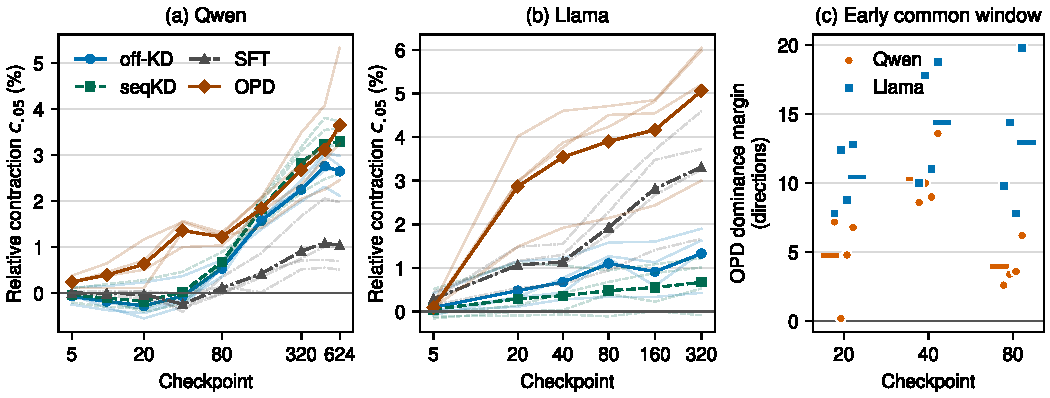
\includegraphics[width=\textwidth]{figures/fig1_main_trajectories.pdf}
\caption{Activation, weight, and functional trajectories. Rows show Qwen and Llama;
columns show activation ER, TPNT excess lift above its null, PABS drift
$10^4(1-\mathrm{PABS})$, and equal-5 relative functional contraction. Column scales have
different units and raw magnitudes are not comparable. Lines connect observed checkpoints
only. Functional contraction exposes training-setting separation not jointly reproduced
by the preceding coordinates.}
\label{fig:main}
\end{figure*}

\begin{table*}[!t]
\centering
\small
\setlength{\tabcolsep}{5pt}
\begin{tabular}{lccc}
\toprule
Model & Activation suite $A$ & Functional $C_5$ & Weight $P_{k,5}$ \\
\midrule
Llama & .556 & \textbf{.743} & .688 \\
Qwen & .595 & \textbf{.708} & .521 \\
\bottomrule
\end{tabular}
\caption{OPD identification on strict common grids (checkpoint-held-out AUC). Each model
uses 64 common states, identical equal-5 modules, and identical folds. $A$ is the
eight-feature activation suite containing ER, PR, top-1/8/32 shares, raw/centered
anisotropy, and step-0 CKA; it is not the single ER trajectory in Figure~\ref{fig:main}.}
\label{tab:identification}
\end{table*}

\begin{table*}[!t]
\centering
\small
\setlength{\tabcolsep}{4pt}
\begin{tabular}{lrrrrr}
\toprule
Model & $M_{\min}^{\mathrm{early}}$ & OPD NCD & SFT NCD & off-KD NCD & seqKD NCD \\
\midrule
Qwen & .200 & \textbf{50.423} & 9.554 & 31.017 & 37.793 \\
Llama & 7.800 & \textbf{77.594} & 39.683 & 17.518 & 11.093 \\
\bottomrule
\end{tabular}
\caption{Shared early ordering and full-trajectory contraction dose.
$M_{\min}^{\mathrm{early}}$ is the minimum continuous OPD margin over four core domains
and shared early checkpoints (directions); positivity excludes a reversal on this grid.
NCD integrates depth and duration through $T=320$ in directions$\times$log-step. The
two columns have different units and are not numerically comparable.}
\label{tab:ncd}
\end{table*}

\begin{figure*}[!t]
\centering
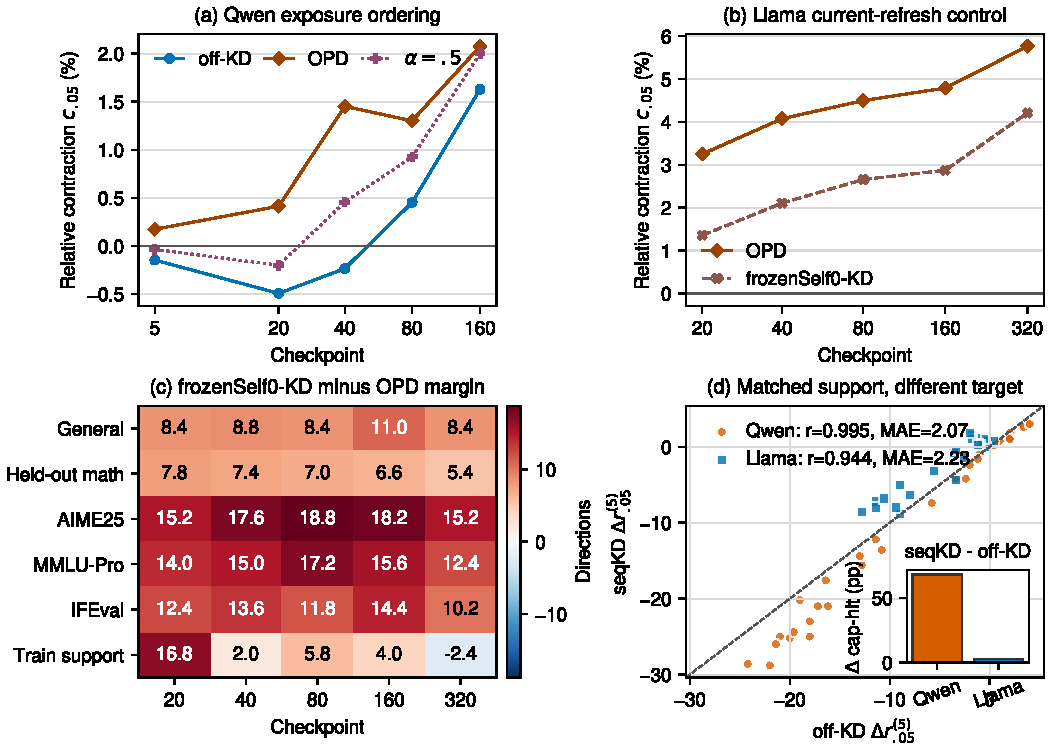
\includegraphics[width=\textwidth]{figures/fig2_support_controls.pdf}
\caption{Sequence-exposure and refresh controls. (a) Ordered Qwen $\alpha=.5$ movement
relative to off-KD and OPD. (b) Mean absolute trajectories of Llama OPD and
frozenSelf0-KD over five fixed external domains. (c) Corresponding paired margins;
positive values indicate deeper contraction under continuously refreshed OPD, and the
thick black line is the external-domain mean. Math, AIME, MMLU, and Mean denote held-out
math, AIME25, MMLU-Pro, and the five-domain mean.}
\label{fig:controls}
\end{figure*}

\begin{table*}[!t]
\centering
\small
\setlength{\tabcolsep}{2.7pt}
\textbf{A. Per-domain equal-5 path agreement, off-KD vs. seqKD
(Pearson $r$/MAE directions)}\\[2pt]
\begin{tabular}{lccccc}
\toprule
Model & General & Math & MMLU-Pro & IFEval & Pooled \\
\midrule
Qwen & .995/1.13 & .996/2.67 & .998/2.18 & .999/2.29 & .995/2.07 \\
Llama & -.771/2.53 & .971/1.73 & .968/2.23 & .824/2.40 & .944/2.23 \\
\bottomrule
\end{tabular}

\vspace{4pt}
\textbf{B. Endpoint behavior for matched-support settings (\%)}\\[2pt]
\begin{tabular}{llrrrrrrr}
\toprule
Model & Setting & \multicolumn{2}{c}{MATH500} & \multicolumn{3}{c}{MMLU-Pro} & \multicolumn{2}{c}{IFEval} \\
\cmidrule(lr){3-4}\cmidrule(lr){5-7}\cmidrule(lr){8-9}
 & & Acc. & Cap & Strict & Flex. & Extract & Prompt & Instr. \\
\midrule
Qwen & off-KD & 79.4 & 4.8 & 35.4 & 57.1 & 47.3 & 23.1 & 36.5 \\
 & seqKD & 72.4 & 73.0 & 30.6 & 58.1 & 54.1 & 24.4 & 39.3 \\
Llama & off-KD & 8.2 & 91.8 & 14.2 & 16.4 & 50.3 & 19.6 & 33.2 \\
 & seqKD & 10.2 & 94.6 & 13.1 & 15.4 & 51.6 & 19.2 & 31.5 \\
\bottomrule
\end{tabular}
\caption{Matched-support functional paths and behavioral readout. A uses matched nonzero
checkpoints; MAE is the checkpoint-wise direction difference. B uses Qwen step 624 and
Llama step 320. Cap denotes generation-cap hit, Extract extraction failure, and
Prompt/Instr. IFEval prompt/instruction strict.}
\label{tab:support-readout}
\end{table*}

\begin{figure*}[!t]
\centering
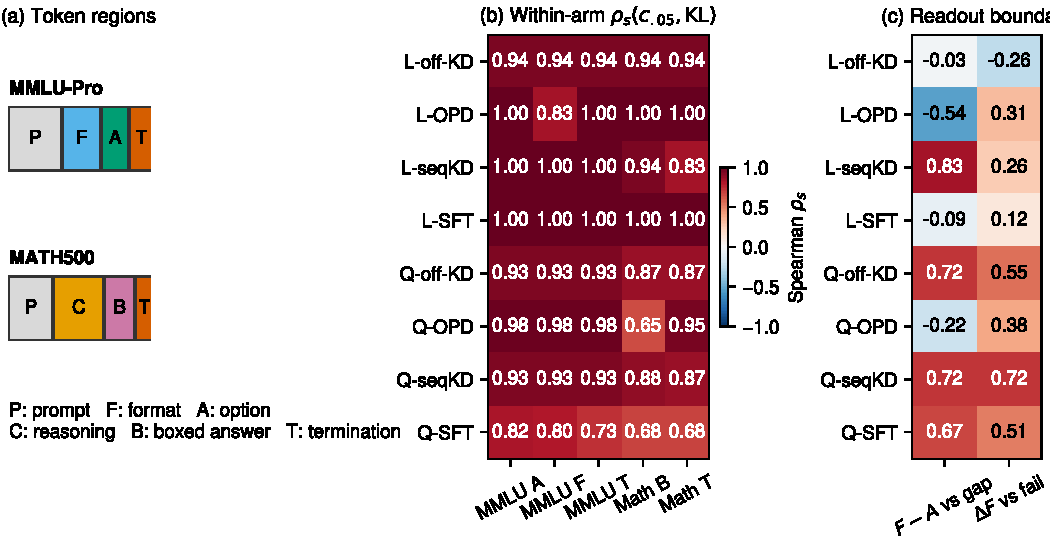
\includegraphics[width=\textwidth]{figures/fig3_regional_output.pdf}
\caption{Regional output relationships. (a) Within-model, within-setting Spearman
correlations between equal-5 functional contraction and regional full-vocabulary KL.
MMLU-Pro columns are format ($F$), correct answer-choice label ($A$), and termination
($T$); MATH500 columns are reasoning ($C$), boxed answer ($B$), and termination ($T$).
(b) MMLU-Pro correlations of the format--answer signed-NLL contrast with the
strict--flexible gap and of format NLL with extraction failure. L and Q denote Llama and
Qwen; each cell prints its correlation.}
\label{fig:regional}
\end{figure*}

\begin{table*}[!t]
\centering
\small
\setlength{\tabcolsep}{4pt}
\begin{tabular}{llcc}
\toprule
Model/domain & Regions & Held-out $R^2$: $C_5$ & Best $P_{k,5}$ \\
\midrule
Llama / MMLU-Pro & $A/F/T$ & \textbf{.869/.932/.468} & .743/.788/.459 \\
Llama / MATH500 & $B/T$ & .561/\textbf{.812} & \textbf{.615}/.647 \\
Qwen / MMLU-Pro & $A/F/T$ & \textbf{.426/.577/.596} & .243/.318/.443 \\
Qwen / MATH500 & $B/T$ & \textbf{.227}/.604 & .167/\textbf{.718} \\
\bottomrule
\end{tabular}
\caption{Out-of-fold prediction of regional full-vocabulary KL. $C_5$ and $P_{k,5}$
use the same five modules, states, and checkpoint-held-out folds. Values follow the
region order; bold marks the higher per-region $R^2$. The later Math $C$ audit is
reported within trajectories and after checkpoint demeaning, but is not included in
this matched held-out table.}
\label{tab:regional-prediction}
\end{table*}


\subsection{Functional Spectra Add Information Beyond Activation and Weight Coordinates}

Figure~\ref{fig:main} places four observables on the same training settings and checkpoints.
ER measures the spectral dimension of activation covariance; TPNT measures enrichment of
update coordinates in a source-principal mask; PABS measures rotation of dominant weight
subspaces; the functional spectrum measures output modes formed by the current weight on
directions actually visited by a domain. Their vertical scales are incomparable, but
their trajectory structure can be compared.

Activation trajectories do not reproduce the functional separation. Across several
external Llama domains, ER changes by less than $.003$ at OPD@160 and step-0 CKA remains
approximately $.9997$--$1.0000$, while $r_{.05}$ at the same locations has fallen by
roughly 14--26 directions. TPNT shows local enrichment above a spectrum-matched null at
some checkpoints but no stable cross-model OPD-specific path. PABS remains close to one,
with small NSS, indicating that these LoRA trajectories evolve largely within a nearly
fixed dominant weight basis. Equal-5 functional contraction, in contrast, clearly
separates the training settings in the last column of Figure~\ref{fig:main}. This
difference comes from the joint action of $W_t$ and the domain input metric, not merely
from adding more features. Native metrics, nulls, and layer results are in Supplementary
Secs.~B.4 and C.3.

We then leave out checkpoint groups on 64 strictly common states per model.
Table~\ref{tab:identification} compares the complete activation suite $A$, functional
contraction $C_5$, and source-principal block $P_{k,5}$. $C_5$ provides stronger OPD
ranking in both models and exceeds raw activations on all three output targets under the
same protocol. Strict $p_k$ retains a local Qwen absolute-NLL advantage, so functional
state and update placement remain task-dependent complements rather than a universal
dominance relation (Supplementary Sec.~D.3).

\subsection{OPD Dominates Shared Early Functional Contraction}

The last column of Figure~\ref{fig:main} shows deeper early OPD contraction in both
models. To test whether domain averaging hides a reversal, define the margin over the
nearest offline setting:
\begin{equation}
M_{m,D,t}
=\min_{b\in\{\mathrm{SFT,offKD,seqKD}\}}\Delta r_{m,b,D,t}^{(5)}
-\Delta r_{m,\mathrm{OPD},D,t}^{(5)}.
\end{equation}
$M>0$ means that OPD contracts more than every offline setting. At
$\varepsilon=.05$, the minimum margin across four core domains and steps 20/40/80 is
positive for both models; complete domain curves are in Supplementary Sec.~C.1. We also
integrate below-base contraction in $\tau=\log(1+t)$ through $T=320$ to obtain negative
contraction dose (NCD). Table~\ref{tab:ncd} keeps early ordering and full-trajectory dose
separate; OPD has the largest NCD in both models.

Four thresholds, continuous spectra, centered covariance, and layer audits preserve this
conclusion. Module audits show that the OPD-deepest ordering is more stable in
value/output and MLP projections, whereas q/k are heterogeneous; this is not an
attribution of contraction energy to five modules. Complete equal-7, layer, and module
results are in Supplementary Secs.~C.2--C.3.

\subsection{Exposure and Refresh Organize Trajectories, Not Readout}

Under the same forward-KL target, Qwen $\alpha=.5$ moves in an ordered direction from
off-KD toward OPD without forming an exact one-dimensional interpolation
(Figure~\ref{fig:controls}a). Llama frozenSelf0-KD instead removes only continual refresh
of current-student rollouts. OPD's contraction advantage persists at all later checkpoints
on five fixed external domains (Figures~\ref{fig:controls}b--c), making the
current-support refresh bundle the more direct organizer. Because refresh jointly changes
rollout length, EOS, repetition, and style, this control identifies the aggregate refresh
bundle rather than a pure freshness effect.

Off-KD and seqKD use identical teacher sequences, order, steps, and LoRA configuration,
changing only the target. Table~\ref{tab:support-readout}A shows highly aligned paths
across all four Qwen domains; Llama mode budgets remain close, although temporal
co-movement is heterogeneous on General. Readout is not locked by these paths. Qwen
seqKD has a much higher endpoint MATH500 cap-hit rate, with accuracy and formatting
changes, while Llama does not reproduce a divergence of comparable size
(Table~\ref{tab:support-readout}B). Matched sequence support can organize a similar
functional-mode budget while target distribution changes its realization.

\subsection{Relative Contraction Tracks Regional Unsigned Movement}

Figure~\ref{fig:regional}a compares $c_{.05}^{(5)}$ with regional KL within each training
setting. Formatting, answer, and termination on MMLU, and reasoning, boxed answer, and
termination on MATH, mostly move with functional contraction. Math CoT is positive in
all four settings of both models. To fix training stage, we subtract the contemporaneous
four-setting mean within each model--domain--checkpoint. Math $\mathrm{KL}_C$ remains
correlated at $.875/.573$ in Llama/Qwen, compared with $.902/.440$ for
$\mathrm{KL}_B$; the regional contrast $\mathrm{KL}_B-\mathrm{KL}_C$ is
$-.209/-.183$. Functional contraction therefore tracks how far each region moves but
does not determine whether movement is allocated primarily to reasoning or final answer.

Table~\ref{tab:regional-prediction} compares $C_5$ with the strong weight baseline
$P_{k,5}$ on the originally frozen actual-KL regions. Functional contraction has higher
held-out $R^2$ in most regions, with explicit exceptions for Llama Math boxed answer and
Qwen Math termination. This matched comparison does not yet include the later Math $C$
audit, so we do not fold the new region into the old win summary. Across signed and
absolute targets the average gap narrows, and the unsigned relation also persists when
the full fixed reference completion is merged into one region (Supplementary
Secs.~D.1--D.3).

\subsection{Signed Readout and Behavior Are Model-Dependent}

KL measures movement magnitude; signed NLL asks whether reference tokens become easier
or harder. MMLU-Pro $\Delta\mathrm{NLL}_{F-A}$ contrasts format and answer, while MATH
$\Delta\mathrm{NLL}_{B-C}$ contrasts boxed answer and preceding reasoning. Their
relationships to strict--flexible gaps or extraction failure change sign across models
and settings (Figure~\ref{fig:regional}b). For example, $F-A$ is positively associated
with the format gap in Qwen off-KD/seqKD but negatively associated in Qwen OPD and Llama
OPD. Functional mode count, regional allocation, reference-token valence, and free
generation are related but non-interchangeable levels.

This boundary agrees with matched support. Functional spectra describe how sequence
support organizes local mode budgets and how far output distributions move, but one rank
cannot determine whether that movement improves or harms a task. Qwen adapter zeroing
and answer-position probability-mass audits further support a formatting/readout-channel
account, but remain model-specific evidence (Supplementary Sec.~D.5).
